\chapter{Method}
\label{cha:method}

The dataset contract in Chapter~\ref{cha:dataset} defines each forecast origin as an aligned combination of plant history, numerical context, and recent satellite imagery. This chapter turns that contract into a sequence of model variants, called arms. Each arm starts from the same numerical lineage and visual source, then changes one part of the visual pathway: its compression, token selection, placement in the sequence, or temporal coverage.

A power trace tells the model what has already happened at a plant, but it does not show a cloud boundary approaching from outside the local measurement. A recent satellite clip may carry that information. It is a dense spatiotemporal field, while the numerical forecaster works with a short sequence of compact tokens. Every arm therefore has to reduce the visual field enough to make computation feasible. It must also keep the location and evolution of the scene parts that could matter for the next hours of production.

\section{Overview and shapes}

The dataset contract supplies every arm with the same forecasting example: fourteen days of normalized power history and numerical covariates. Single-anchor visual arms use one eight-frame satellite clip recorded before the forecast origin. Each multi-anchor arm uses five such clips at distinct daily anchors. Horizon weather covariates are archived measurements used as proxies for forecasts, as defined in the problem setting in Chapter~\ref{cha:intro}. For the primary United Kingdom track, that fourteen-day history contains 672 half-hour observations and the forecast covers the next 12 observations, or six hours. Each forecast returns nine quantiles at every lead time, allowing the model to express a wider interval when the next cloud evolution is uncertain.

The arms form a ladder of increasingly direct visual access. The numerical baseline receives no images. The pooled-image baseline reduces the visual field to a learned summary before fusion. Spatial-token fusion retains selected locations and inserts them into the recent numerical sequence. Multi-anchor applies the same idea at five daily anchors. Full payload is a separate extension that retains the full spatial-token payload at each anchor. The standard ladder arms share the partition, forecast origins, loss, and scoring rules. The full payload extension uses only origins with all five cached entries, as described in its subsection. Differences in dropout and mask handling are retained in the training recipe because they affect how individual comparisons should be read.

Table~\ref{tab:fusion-ladder-design} summarizes the four ladder arms and the full payload extension before the sections below describe their shared components and individual pathways.

\begin{table}[htbp]
\centering
\begin{tabularx}{\textwidth}{@{}lYYY@{}}
\hline
Arm & Visual input & Placement & Role \\
\hline
Numerical & None & None & Numerical control \\
Pooled-image & Learned summary & Auxiliary row & Summary bottleneck \\
Spatial-token & 98 spatial tokens & Recent context & Spatial access \\
Multi-anchor & 20 tokens/anchor & Five daily patches & Repeated daily evidence \\
Full payload & 98 tokens/anchor & Five daily patches & Detailed daily views \\
\hline
\end{tabularx}
\caption{Fusion ladder. The standard arms change how the same satellite source reaches the forecaster. The full payload extension is evaluated on origins with all five required cached entries.}
\label{tab:fusion-ladder-design}
\end{table}

The representations in Table~\ref{tab:token-budgets} determine the sequence length seen by attention. Chronos-2 groups the 672 half-hour context values into $T_{\mathrm{ctx}}=\lceil672/16\rceil=42$ numerical patches. A single future-query token requests all 12 lead times, and the quantile head returns $[B,12,9]$ for batch size $B$.

\begin{table}[htbp]
\centering
\begin{tabular}{@{}lccc@{}}
\hline
Arm & Context + query & Visual tokens & Row length \\
\hline
Numerical & $42+1$ & None & 43 \\
Pooled-image & $42+1$ & 1 (auxiliary row) & 43 \\
Spatial-token & $42+1$ & 98 (one anchor) & 141 \\
Multi-anchor & $42+1$ & $20\times5$ & 143 \\
Full payload & $42+1$ & $98\times5$ & 533 \\
\hline
\end{tabular}
\caption{Target-row token budgets of the numerical and visual arms. The pooled-image baseline has a 43-position target row and a separate one-position visual row; it is therefore not a 44-position temporal sequence.}
\label{tab:token-budgets}
\end{table}

Multi-anchor has a similar target-row length to spatial-token fusion, although it distributes 100 visual tokens across five anchors instead of placing 98 at one recent anchor. The full payload extension expands that budget to 490 visual tokens across the same five anchors.

The pooled-image baseline compresses the 784 cells in the cached visual field to one learned summary before the numerical forecaster receives visual information. That summary is computed independently of the numerical state, and its auxiliary row cannot preserve an addressable image location. Spatial-token fusion retains 98 selected cells with their spatial identity. The later results therefore test whether that direct access to selected visual locations matters more than a global learned summary.

\section{Design principle: decoupled resolution}
\label{sec:decoupled}

The numerical and visual sources are intentionally kept at different resolutions. The numerical branch has a long fourteen-day history because it must infer daily structure and the recent behaviour of an unfamiliar plant. The visual branch has eight high-cadence frames near the forecast origin because it is intended to describe recent cloud evolution. Resampling the power history to image cadence would obscure the long context that supports cross-plant transfer. The architecture joins the two sources only after each has been represented at the resolution appropriate to its task.

\section{Shared numerical backbone: Chronos-2}

Every arm uses the same Chronos-2 numerical backbone. Visual-arm initialization follows the seed-matched numerical baseline defined below; the recipe and mask differences remain part of each comparison. This section describes the shared path from the fourteen-day numerical history to the quantile forecast.

Chronos-2 receives normalized power history and the numerical covariates permitted at the forecast horizon. It groups the 672 historical values into non-overlapping patches of 16, producing 42 context tokens that each span eight hours. A further position represents the future patch to predict. Patching preserves the full fourteen-day history without requiring attention over every half-hour observation.

The loaded checkpoint has width 768, twelve encoder blocks, twelve attention heads, and a 3072-dimensional feed-forward layer. These checkpoint dimensions are retained during loading. In the visual arms, the pretrained numerical backbone is frozen except for the shared quantile head, the new fusion components, and the final three encoder blocks. Those trainable components give the visual pathway a route into the forecast while retaining most of the representation learned by the numerical baseline. Within each block, temporal attention relates positions in the history, and group attention relates the target and covariate rows. The feed-forward layer updates their representations. The quantile head reads the final target representation and predicts all 12 horizon steps together.

The method proceeds from the numerical baseline to visual pathways with progressively less compression, all built on this shared backbone.

\section{Numerical baseline}

The numerical baseline is the vision-free control and seed-specific initialization for the visual arms.

The numerical baseline is trained first. Each visual arm starts from the numerical checkpoint with the matching random seed. Its bridge is therefore learned on top of a forecaster already adapted to the training plants. Figure~\ref{fig:mmtsfm-s1} shows this numerical path without a visual stack.

\begin{figure}[H]
\centering
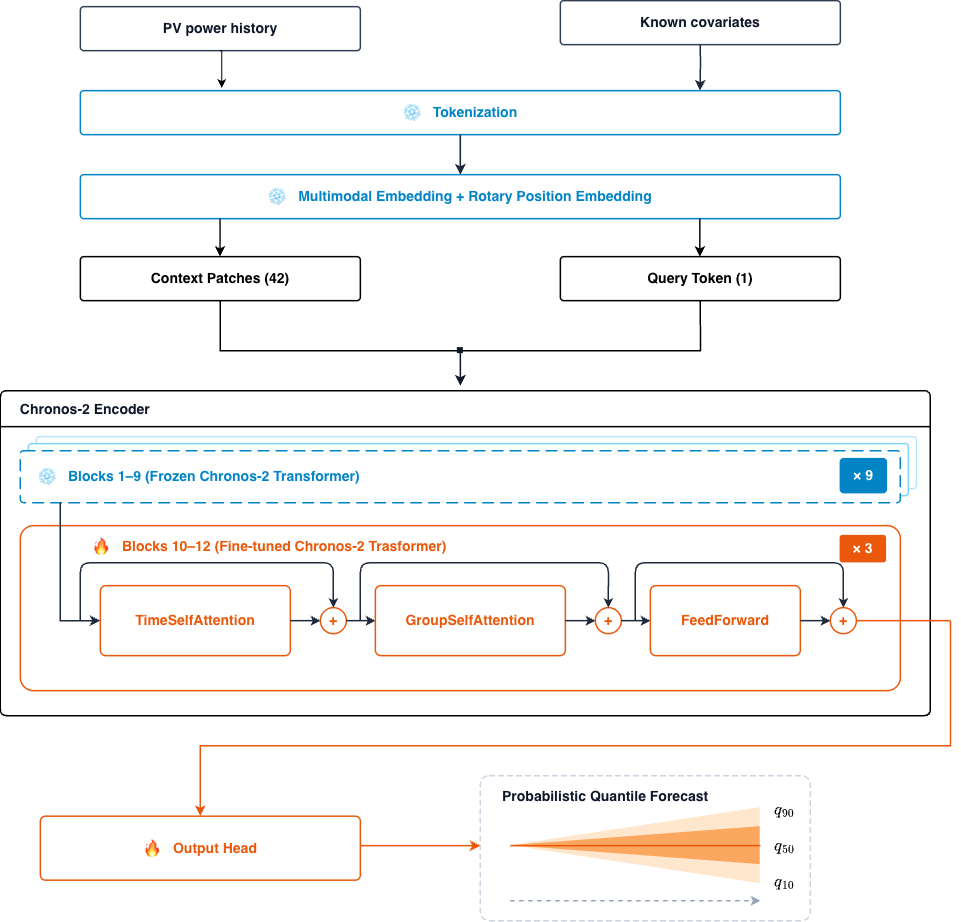
\includegraphics[width=0.90\textwidth]{figures/mmtsfm_s1.png}
\caption{Power history and numerical covariates are converted into temporal tokens and processed by Chronos-2. This arm has no image input and provides the common starting point for the visual arms.}
\label{fig:mmtsfm-s1}
\end{figure}

This first stage adapts the inherited forecasting components on the training plants, starting from general time-series pretraining rather than random weights. The resulting seed-specific checkpoint is the learned numerical base passed to every later arm.

\section{Shared visual backbone: frozen V-JEPA 2.1}

The visual encoder is shared by every visual arm and is never trained, so it is described once here. Its latent geometry, mismatch with the numerical sequence, and cached execution determine the visual interfaces that follow.

The visual pathway begins with V-JEPA 2.1 ViT-L/16. It processes the eight-frame satellite clip as a short video rather than as eight unrelated images. The encoder produces four temporal latent slices. Each slice contains a 14 by 14 grid of spatial patches, giving 196 patch features of width 1024. The complete visual representation therefore has the shape $[B,4,196,1024]$.

A video encoder is chosen on the expectation that sky evolution carries forecasting information.

The visual latents are extracted before model training and read from a cache. Repeated seeds and multi-anchor layouts are feasible because the video encoder does not run in every training step. The visual-validity mask travels with the cached features. A missing frame is therefore represented as missing evidence, not as a synthetic clear-sky image. The architecture can continue from numerical evidence when the image clip is incomplete.

\section{Pooled-image baseline, late fusion through a learned bottleneck}

The pooled-image baseline tests whether one learned visual summary helps Chronos-2 while leaving its numerical sequence unchanged. A causal Perceiver-style resampler~\cite{perceiver} attends over the V-JEPA patch field and produces one learned summary token. The cross-modal adapter projects it to Chronos-2's 768-dimensional width and places it on an auxiliary visual row. Group attention processes this row with the numerical rows.

Figure~\ref{fig:mmtsfm-s2a} follows the visual field through this bottleneck.

\begin{figure}[H]
\centering
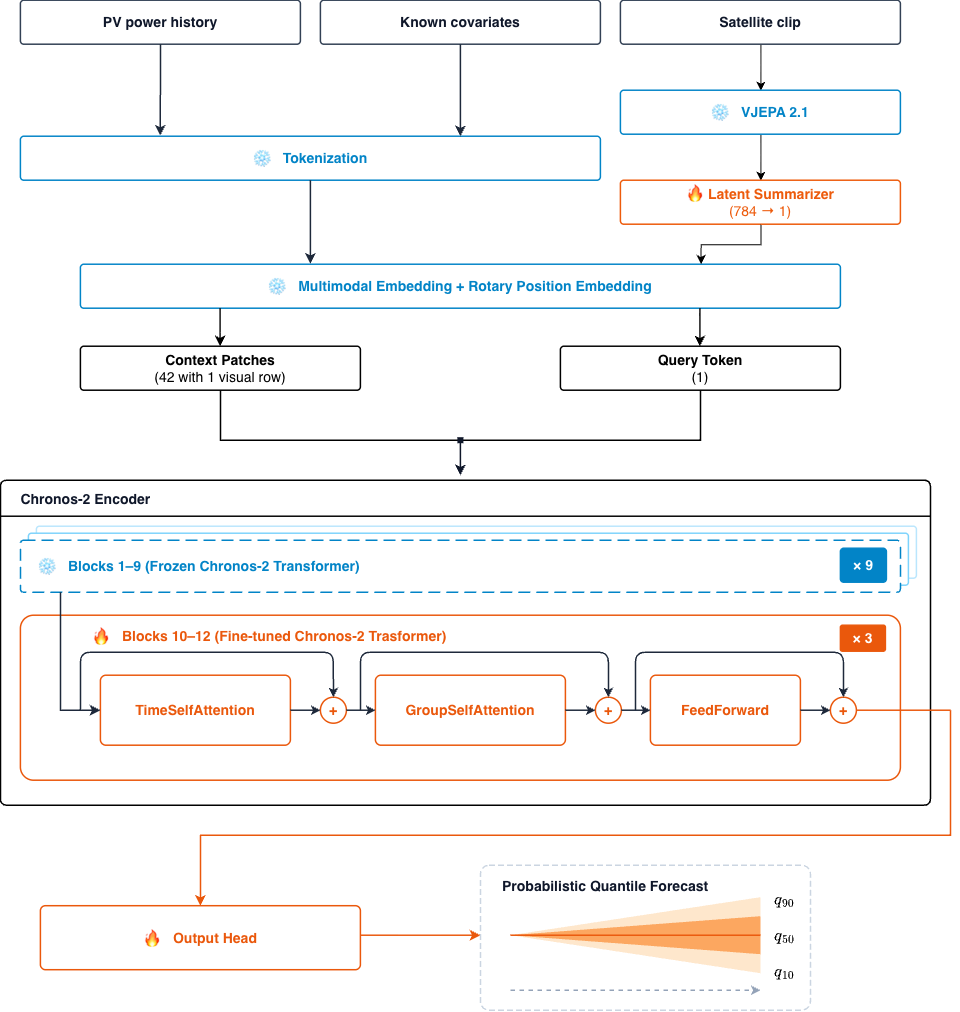
\includegraphics[width=0.92\textwidth]{figures/mmtsfm_s2a.png}
\caption{Pooled-image baseline. The learned resampler converts the complete visual field into one summary token, which enters Chronos-2 as a separate visual row.}
\label{fig:mmtsfm-s2a}
\end{figure}

The resampler maps 784 patch cells to one token, so spatial locations are not exposed as separate entries to later layers. The baseline tests whether this global summary carries enough information before the next arm preserves selected locations as addressable tokens.

\section{Spatial-token fusion, single-anchor interleaving}

Spatial-token fusion replaces the pooled-image baseline's global summary with selected visual tokens. Those tokens are inserted into the final numerical context patch, where the shared encoder can process them with the recent power history. This arm introduces the resampler-free path at one anchor.

The visual pruning and interleaving draw inspiration from the visual-token pathway in Nemotron 3 Nano Omni~\cite{nemotron}, discussed in Section~\ref{sec:rw-nemotron}. Its spatial reduction and token selection motivate keeping a compact set of spatially distinct visual features. Here, that idea is adapted to forecasting: selected visual tokens are interleaved at their observation times with the numerical sequence, so the shared temporal encoder can process both sources together.

The visual field first undergoes a $2\times2$ spatial-to-channel rearrangement. Each block of four neighboring patches in the original 14 by 14 grid becomes one cell, leaving a 7 by 7 field of 49 cells. Concatenating the four 1024-dimensional patch features gives each cell 4096 features. A projector then maps each cell to Chronos-2's 768-dimensional width. Selection retains the 49 cells from the first temporal slice, ranks later cells by cosine change from the preceding slice, and retains 49 additional candidates. The resulting 98 tokens enter the numerical sequence at their observation positions. The tensor path is $[B,4,196,1024]$ for the cached field, $[B,4,49,4096]$ after rearrangement, and $[B,98,768]$ after projection and selection, where $B$ is the number of forecast examples processed together. The other axes denote temporal slices, spatial cells, and feature dimensions before selection; afterward, the middle axis counts selected tokens. The final tensor is interleaved with 42 numerical context tokens and one future-query token.

The projector matches the visual width to the numerical width without mixing information across image locations. A learned coordinate embedding identifies each of the 49 cells, while the sequence position records its observation time. The model can therefore distinguish where a change occurred from when it was observed.

Figure~\ref{fig:mmtsfm-s2d} shows the reduction, selection, and interleaving path.

\begin{figure}[H]
\centering
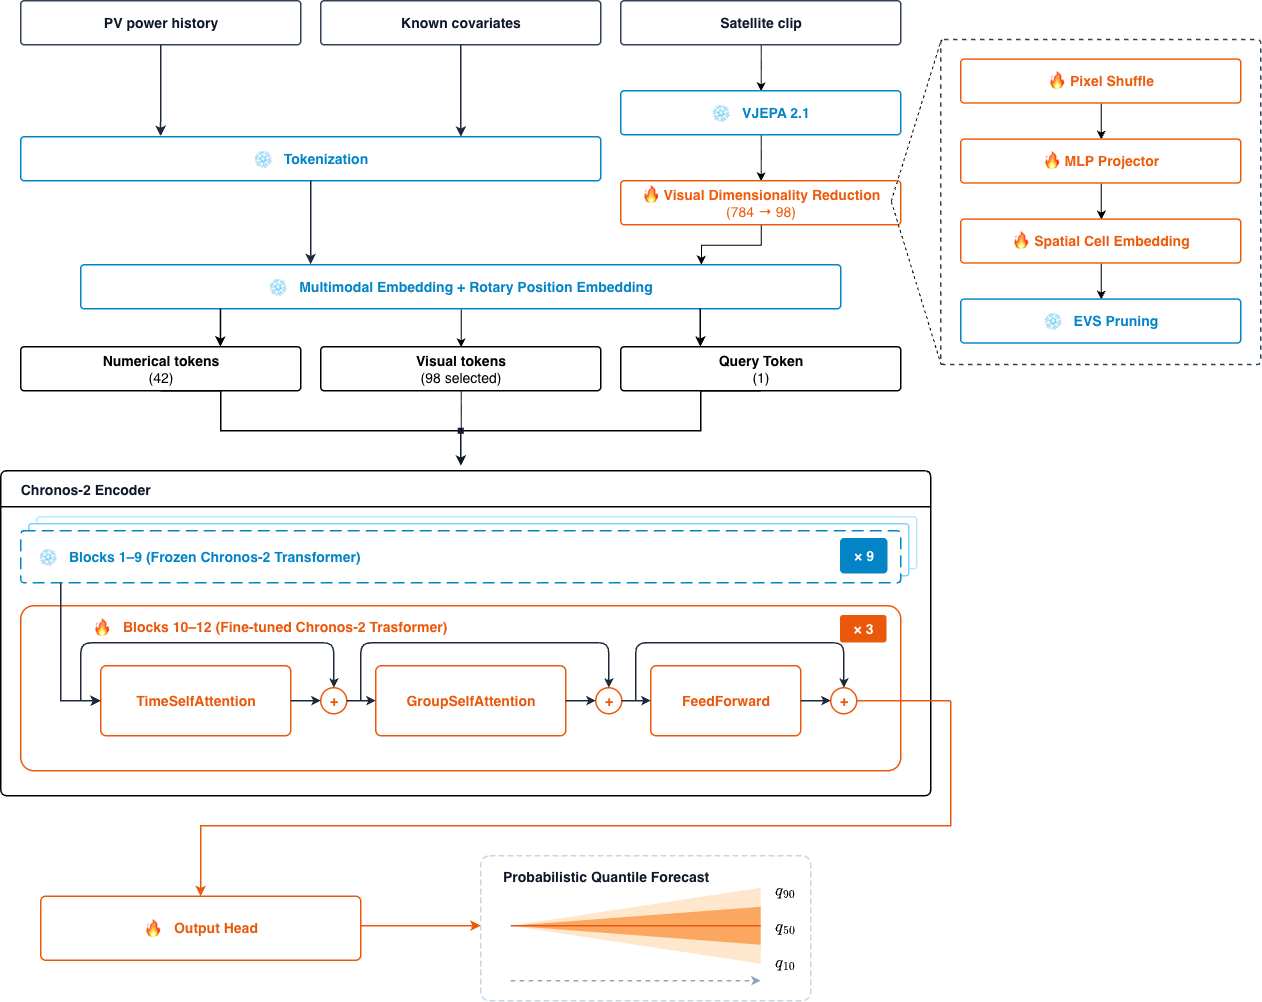
\includegraphics[width=0.96\textwidth]{figures/mmtsfm_s2d.png}
\caption{Spatial-token fusion, resampler-free interleaved fusion. Forty-two numerical context tokens, 98 selected visual tokens, and one query form a 141-position target row. Visual cells are reduced spatially, projected, selected by temporal change, and interleaved at their observation positions.}
\label{fig:mmtsfm-s2d}
\end{figure}

The cached field contains 196 cells: 49 spatial cells in each of four latent slices. All 49 cells from the first slice are retained as an anchor field. The remaining 147 cells are ranked by cosine dissimilarity from the corresponding cell in the preceding slice, and the highest-scoring 49 complete the 98-token payload.

The selected tokens take positions associated with their observation times inside the final numerical context patch, producing the 141-position sequence in Table~\ref{tab:token-budgets}. The shared temporal mixer processes visual and numerical tokens together, so a retained visual location can affect the numerical representation in every encoder block. The arm has no pooled-image resampler or adapter, so the selected locations remain directly available to the encoder.

\section{Multi-anchor}

Multi-anchor extends spatial-token fusion from one recent anchor to five anchors, one on each of five consecutive days. The anchors share the same clock time, so their solar geometry is broadly comparable. The model can then see several examples of the relation between local sky appearance and power at that time of day.

Each daily anchor is represented by a cached clip whose four temporal latent slices are available to the encoder. For multi-anchor, the selector compares two successive slices from that cached representation and retains both endpoints for each selected spatial trajectory. These two slices describe one anchor; they do not create two additional daily anchors.

Figure~\ref{fig:mmtsfm-s2e} shows where the five visual blocks enter the numerical history.

\begin{figure}[H]
\centering
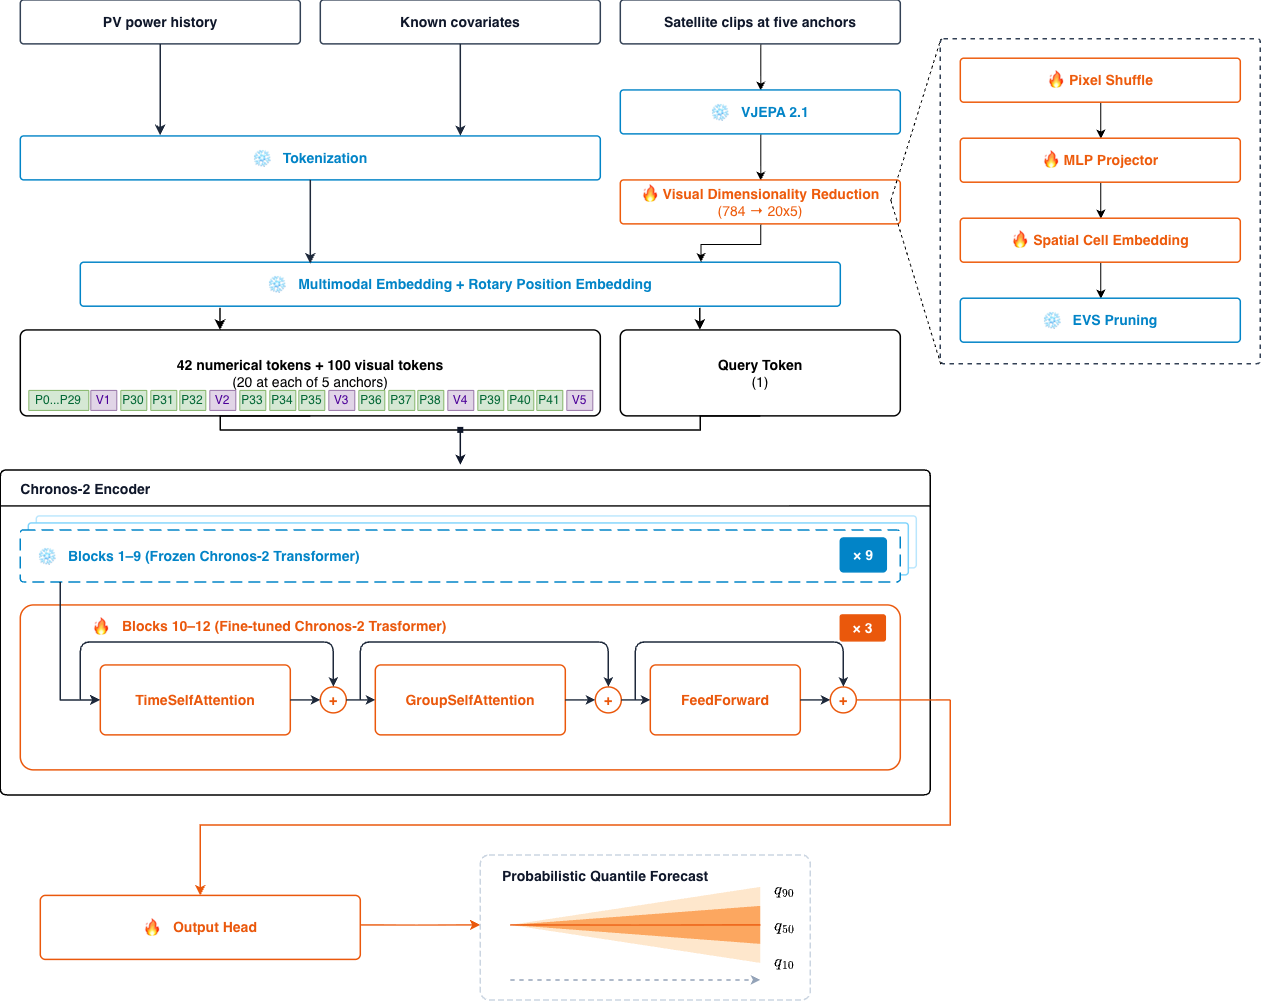
\includegraphics[width=\textwidth]{figures/mmtsfm_s2e.png}
\caption{Multi-anchor. Five blocks of 20 visual tokens are interleaved with 42 numerical context tokens and one query, forming a 143-position target row. Each block represents one daily anchor.}
\label{fig:mmtsfm-s2e}
\end{figure}

Within each anchor, the paired-novelty selector ranks the 49 spatial trajectories by cosine change between the two slices. It retains both endpoints for the ten most-changing trajectories. This yields 20 tokens per anchor and 100 tokens overall.

Each visual block shares the integer position of the numerical patch at its daily anchor. The resulting sequence has 42 numerical context tokens, 100 visual tokens, and one future-query token, for a total of 143 positions as shown in Table~\ref{tab:token-budgets}.

\section{What each arm reuses and what it learns}

The arms share numerical and visual foundations and differ through the visual bridge. Distinguishing inherited components from newly trained ones makes the comparison boundary explicit and clarifies which parts can account for differences in outcome.

Every arm loads the same Chronos-2 components (patch tokenizer, twelve encoder blocks, positional machinery, group attention, and multi-quantile head). Visual-arm initialization follows the numerical-baseline procedure above. Each arm also reads the same pretrained V-JEPA latents from cache. The video encoder never runs inside the training loop, so image augmentation, crop changes, and visual-backbone gradients are outside the training process. The bridge built on top distinguishes the visual arms, as summarized in Table~\ref{tab:trainable-parts}.

\begin{table}[htbp]
\centering
\begin{tabularx}{\textwidth}{@{}lY@{}}
\hline
Arm & Components \\
\hline
Numerical & None; inherited components adapted \\
Pooled-image & Causal summarizer, cross-modal adapter, shared head \\
Spatial-token & Projector, modality embeddings, shared head \\
Multi-anchor & Projector, integer positions, shared head \\
\hline
\end{tabularx}
\caption{Newly initialized and trainable components by arm. The visual encoder remains frozen; the final three Chronos-2 blocks and shared quantile head train in visual arms.}
\label{tab:trainable-parts}
\end{table}

The ladder is a controlled comparison of visual interfaces, not a claim that every training detail is identical. Table~\ref{tab:comparison-boundaries} separates the common conditions from the choices that still vary and must therefore remain part of the interpretation.

\begin{table}[htbp]
\centering
\begin{tabularx}{\textwidth}{@{}lYY@{}}
\hline
Aspect & Shared & Varies \\
\hline
Evaluation & Plant split, horizon, scoring & - \\
Initialization & Seed-matched Chronos-2 warm start & Bridge and trainable parameters \\
Vision & V-JEPA cache and validity mask & Pooling, selection, anchor count \\
Sequence & 42 context patches + one query & Auxiliary row or interleaved tokens \\
Training & Frozen V-JEPA; final three Chronos blocks trainable & Visual dropout, numerical masks \\
\hline
\end{tabularx}
\caption{Comparison boundaries for the fusion ladder.}
\label{tab:comparison-boundaries}
\end{table}

\section{Computational scaling of the interfaces}

The visual information retained by each arm also determines the work required of the shared transformer. This section compares sequence sizes and then describes the per-sample forward path.

Sequence length sets the main attention cost. Self-attention compares pairs of positions, so its activation cost grows approximately with the square of the sequence length. Spatial-token fusion has 141 positions, compared with 43 for the numerical baseline target row, and therefore has about 10.8 times as many position pairs. Multi-anchor has a similar cost at 143 positions.

\begin{table}[htbp]
\centering
\begin{tabularx}{\textwidth}{@{}lccY@{}}
\hline
Arm & Length & Relative pairs & Memory \\
\hline
Numerical & 43 & 1.0 $\times$ & Reference \\
Spatial-token & 141 & 10.8 $\times$ & Spatial tokens; smaller batches \\
Multi-anchor & 143 & 11.1 $\times$ & Distributed anchors \\
\hline
\end{tabularx}
\caption{Approximate pair-count scaling relative to the 43-position numerical baseline target row. The values describe sequence geometry, not measured end-to-end runtime.}
\label{tab:attention-scaling}
\end{table}

Sending all 784 visual candidates beside the numerical sequence would make the row longer still, especially with more than one anchor. The visual field must therefore be summarized or selected before it enters attention. The pooled-image baseline learns that compression, whereas spatial-token fusion and multi-anchor retain a fixed number of selected cells.

\section{From one dataset window to one forecast}
\label{sec:forward-walkthrough}

A forecast example in the primary UK setting illustrates data construction, arm-specific token assembly, model fitting, and inference. The same sequence applies to validation and test windows within their plant partitions.

Table~\ref{tab:forecast-information} distinguishes inputs tied to the forecast origin from fields available later in the window. Power history and satellite frames come from observations at or before the origin. Calendar and solar geometry are known over the horizon; archived atmospheric measurements are supplied there as proxies for weather forecasts. Future power is reserved for training and evaluation.

\begin{table}[htbp]
\centering
\begin{tabularx}{\textwidth}{@{}lYY@{}}
\hline
Input & Availability & Use \\
\hline
Power history & Observed before origin & Numerical context \\
Satellite & Strictly before origin & Timestamp-matched frames \\
Calendar/solar & Deterministic & History + horizon \\
Weather & Archived horizon observations & Forecast proxy \\
Future power & Unavailable & Masked target; evaluation reference \\
\hline
\end{tabularx}
\caption{Information available to a forecast window.}
\label{tab:forecast-information}
\end{table}

\subsection{Constructing the numerical and visual inputs}

For the primary UK track, the loader resolves fourteen days of half-hourly power history and the following six-hour target window. It works in timestamp space, so missing intervals remain at their physical times instead of shifting later samples forward. Installed capacity converts measured power to the normalized target. Power history, covariate rows, and future targets retain separate validity masks. A measured zero remains an observation, while a missing patch remains unavailable context. The target mask also excludes invalid future values from training loss and evaluation.

The numerical input contains a power row and covariate rows. Calendar and solar-geometry values are known through the forecast horizon. Archived meteorological measurements are also supplied across the horizon as proxies for operational weather forecasts. Chronos-2 patches the 672 historical power samples into 42 tokens. Covariate rows share a group identifier with the power row. Group attention then relates the variables after temporal encoding.

For a visual arm, the plant identifier and frame timestamps link the forecast origin to the satellite observations for that location. Frames are selected before the origin using the timestamp-matching rule described in the dataset chapter. Their precomputed V-JEPA 2.1 representations are then retrieved. The frozen visual encoder processes each clip before forecaster fitting, so its output can be reused across training epochs. Each eight-frame clip supplies four temporal latent slices, each containing a 14 by 14 grid of 1024-dimensional patch features. If a frame or cached representation is unavailable, the corresponding visual validity mask marks it missing; no artificial image is substituted.

\subsection{Building the model sequence}

Every arm starts with 42 numerical context tokens and one future-query token. The numerical baseline sends these rows through Chronos-2 without images. It provides the adapted weights used to initialize the visual arms, with a separate checkpoint for each random seed.

The pooled-image baseline sends the cached patch field to a causal Perceiver-style resampler. The resampler condenses its 784 patch cells to one learned summary, and a cross-modal adapter maps that vector to Chronos-2's 768-dimensional width. The summary enters on an auxiliary visual row in the same group as the numerical rows. Group attention can combine the summary with power and covariates while the 43-position target row stays unchanged.

Spatial-token fusion keeps selected locations as separate entries. A $2\times2$ spatial-to-channel rearrangement combines each block of four neighboring patches into one of 49 cells. A projector maps each 4096-dimensional cell to the 768-dimensional Chronos-2 width. The selector retains all 49 cells from the first latent slice, then ranks cells from later slices by cosine change relative to the preceding slice and selects 49 additional candidates. Their coordinate embeddings identify the spatial cells, while sequence positions identify observation times. The resulting 98 visual tokens enter the target row at those times, giving the row 141 positions including numerical context and query.

Multi-anchor applies paired-novelty selection independently at each daily anchor. It ranks the 49 spatial trajectories by the change between two latent slices. It retains both endpoints for the ten most-changing trajectories. This gives 20 tokens per anchor and 100 overall. Each block is placed at the numerical patch for its anchor. Full payload uses the single-anchor selector at every daily anchor. It contributes 98 tokens per anchor and 490 overall. Its target row has 533 positions.

After assembly, temporal attention processes positions along each row, while group attention relates the target, covariate, and, for pooled-image fusion, auxiliary visual rows. In the interleaved arms, spatial tokens share the target row with numerical context and are processed through the same temporal blocks. The future-query token contains no future target value. It carries the request for all twelve forecast steps through the encoder, so later predictions do not consume earlier generated predictions.

\subsection{Fitting the arms}

Training proceeds in two stages. The numerical baseline adapts Chronos-2, including its quantile head, on training-plant windows and supplies a seed-specific checkpoint. Each visual arm then initializes from the checkpoint with the matching seed. The cached V-JEPA encoder remains frozen; the arm-specific bridge, shared quantile head, and final three Chronos-2 blocks train on the masked quantile objective. The target mask removes invalid future values, and the objective averages pinball loss over valid target steps and the nine quantile levels, as defined in Section~\ref{sec:metric-definitions}. During fitting, visual and numerical dropout expose the visual arms to missing inputs, ensuring that the model maintains forecasting capabilities when visual observations are unavailable.

\subsection{Inference and scoring}

At inference, the selected checkpoint receives a window assembled by the same timestamp and mask rules. For an unseen plant, the model uses its fourteen-day history, covariates, and any available pre-origin visual frames without updating its weights on that plant. Missing visual slots remain masked, so the numerical pathway can still produce a forecast when an image is unavailable.

The encoder processes the assembled sequence once. Its future-query representation feeds the quantile head, which returns a tensor of shape $[B,12,9]$: $B$ forecast examples, twelve half-hour leads, and nine quantile levels from 0.1 through 0.9. The median supplies the point forecast; the full quantile set supports interval, CRPS, and calibration measures. The model does not impose monotonic ordering or apply post-hoc rearrangement, so predicted quantiles are not guaranteed to increase with their stated probability. Training loss and evaluation metrics use the validity masks, with plant weighting and ramp selection specified in Chapter~\ref{cha:protocol}.

The vision-on/off control reruns this same inference pass with visual embeddings set to zero while retaining the fitted weights, numerical embeddings, token positions, origins, and masks. Its score difference tests whether a trained forecast depends on its visual pathway. Stale-image and wrong-plant substitutions test whether that dependence is tied to recent, site-specific content; the intervention details and limits appear in Chapter~\ref{cha:ablations}.

\section{Training recipe}
\label{sec:training-recipe}

The fitting procedure for the baseline and visual arms is described above. This section specifies the learning-rate schedule and modality-dropout settings relevant to comparisons among them.

The visual projector uses a 500-step learning-rate warm-up. Warm-up changes the learning rate at the start of training; it does not change which parameters are trainable. Lightning~\cite{lightning} and Hydra~\cite{hydra} manage the configuration, and training uses distributed bf16 execution on Leonardo HPC.

Modality dropout exposes visual arms to missing inputs during training. The pooled-image baseline uses visual dropout of 0.3 and numerical dropout of 0.1. The interleaved arms use visual dropout of 0.5 and the same numerical dropout.

\section{Implementation and compute}

Hydra composes dataset, model, stage, trainer, logger, and ablation settings; command-line overrides identify each arm and seed. Lightning manages fitting, validation, checkpointing, and testing. The data module constructs plant-disjoint windows, and the model module applies masked quantile loss and exports protocol metrics. Gradient accumulation reduces the per-step GPU batch while retaining an effective batch of sixteen. The training entry point distinguishes a weights-only warm start from a full-state resume. Weights \& Biases records training metrics through Lightning; it runs offline on Leonardo compute nodes, with resolved configurations saved at run start for later synchronization.

Experiments used one or more 64 GB NVIDIA A100 GPU per training job with mixed bfloat16 precision. Frozen V-JEPA 2.1 latents were extracted to a separate cache before model fitting, so the video encoder did not process source frames at every optimization step. The default microbatch of four with four accumulation steps exceeded available device memory for full payload. That arm used a microbatch of two with eight accumulation steps to keep the effective batch at sixteen. The shorter arms used the standard setting.

Table~\ref{tab:compute-budget} reports the mean elapsed runtime for each stage across completed runs on a single NVIDIA A100 GPU. These numbers record observed execution time, whereas the scheduler wall-time limits were set higher to allow for checkpoints and queue timeouts.

\begin{table}[htbp]
\centering
\begin{tabular}{@{}lc@{}}
\hline
Job & Mean elapsed time \\
\hline
V-JEPA latent extraction & 7 h \\
Numerical & 18 h \\
Pooled-image & 20 h \\
Spatial-token & 22 h \\
Multi-anchor & 23 h \\
Full payload & 45 h \\
Evaluation & 30 min \\
\hline
\end{tabular}
\caption{Mean elapsed execution time on a single NVIDIA A100 GPU across completed runs.}
\label{tab:compute-budget}
\end{table}

\section{Full payload}

The multi-anchor arm distributes a fixed visual budget across five days. The full payload arm removes this budget constraint and tests the effect of retaining the full visual detail available to the single-anchor pathway at each daily anchor.

Full payload is a separate high-capacity arm that tests the upper end of the multi-anchor design. It retains five daily anchors, spaced 24 hours apart, and gives each anchor the full spatial-token fusion payload: eight input frames, four temporal latents, and 98 selected visual tokens. The arm therefore supplies five detailed examples of the local sky-power relationship instead of distributing a 100-token budget across five anchors. Its sequence contains 42 numerical context tokens, 490 visual tokens, and one future-query token, for a total of 533 positions.

The arm tests whether retaining more visual detail at each anchor helps the model exploit repeated daily evidence. Visual payload and sequence length increase together, leaving the effect of retaining more detail coupled with added sequence capacity. Attention has about fourteen times as many position pairs as in spatial-token fusion, and training takes longer. The larger interface therefore adds capacity alongside visual evidence.

The arm reuses existing full-depth cached representations, avoiding a new forty-frame video encoding for every forecast origin. For an origin at time $t$, the loader reads cached embeddings across the five daily origins from $t-96$ to $t$ hours, excluding forecast windows where any of the five daily anchors is missing.

Memory, rather than cache storage, is the limiting factor. The default microbatch of four examples with four accumulation steps exhausts a 64 GB A100. The launch therefore uses a microbatch of two with eight accumulation steps, preserving the effective batch size of 16 while reducing the memory required by each forward pass. This adjustment is necessary to run the arm, and it is another reason to interpret it as a separate high-capacity experiment rather than as a direct replacement for the shorter fusion interfaces.
